\documentclass{article}
\usepackage{graphicx}
\usepackage{tikz}
\usetikzlibrary{shapes,arrows}
\usepackage{listings}
\usepackage[margin=1in]{geometry}
\usepackage{color}

% Define colors for code highlighting
\definecolor{codegreen}{rgb}{0,0.6,0}
\definecolor{codegray}{rgb}{0.5,0.5,0.5}
\definecolor{codepurple}{rgb}{0.58,0,0.82}

% Configure code listing style
\lstdefinestyle{mystyle}{
    commentstyle=\color{codegreen},
    keywordstyle=\color{blue},
    stringstyle=\color{codepurple},
    basicstyle=\ttfamily\small,
    breakatwhitespace=false,         
    breaklines=true,                 
    captionpos=b,                    
    keepspaces=true,                 
    numbersep=5pt,                  
    showspaces=false,                
    showstringspaces=false,
    showtabs=false,                  
    tabsize=4
}
\lstset{style=mystyle}

\title{TCP File Transfer Implementation Report}
\author{Truong Xuan Hieu-22BI13163}
\date{\today}

\begin{document}
\maketitle

\section{Protocol Design}
The file transfer protocol is designed as a simple client-server architecture operating over TCP/IP. The protocol follows these steps:

\begin{figure}[ht]
\centering
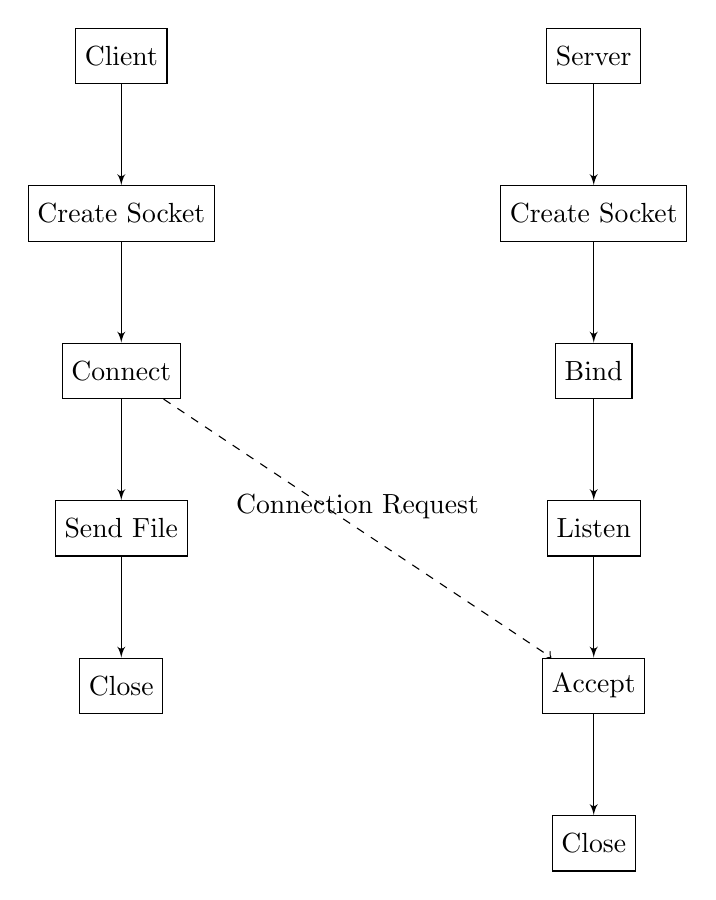
\begin{tikzpicture}[node distance=2cm]
    % Define styles
    \tikzstyle{block} = [rectangle, draw, text centered, minimum height=2em]
    \tikzstyle{line} = [draw, -latex']
    
    % Client side
    \node [block] (client) {Client};
    \node [block, below of=client] (csocket) {Create Socket};
    \node [block, below of=csocket] (connect) {Connect};
    \node [block, below of=connect] (send) {Send File};
    \node [block, below of=send] (cclose) {Close};
    
    % Server side
    \node [block, right of=client, xshift=4cm] (server) {Server};
    \node [block, below of=server] (ssocket) {Create Socket};
    \node [block, below of=ssocket] (bind) {Bind};
    \node [block, below of=bind] (listen) {Listen};
    \node [block, below of=listen] (accept) {Accept};
    \node [block, below of=accept] (sclose) {Close};
    
    % Connect components
    \path [line] (client) -- (csocket);
    \path [line] (csocket) -- (connect);
    \path [line] (connect) -- (send);
    \path [line] (send) -- (cclose);
    
    \path [line] (server) -- (ssocket);
    \path [line] (ssocket) -- (bind);
    \path [line] (bind) -- (listen);
    \path [line] (listen) -- (accept);
    \path [line] (accept) -- (sclose);
    
    % Connection line
    \draw [dashed, ->] (connect) -- node[above] {Connection Request} (accept);
\end{tikzpicture}
\caption{TCP File Transfer Protocol Flow}
\label{fig:protocol}
\end{figure}

\section{System Organization}
The system is organized into two main components as shown in Figure \ref{fig:organization}:
\begin{itemize}
    \item Server Component: Handles incoming connections, receives files
    \item Client Component: Initiates connection, sends files
\end{itemize}

\begin{figure}[ht]
\centering
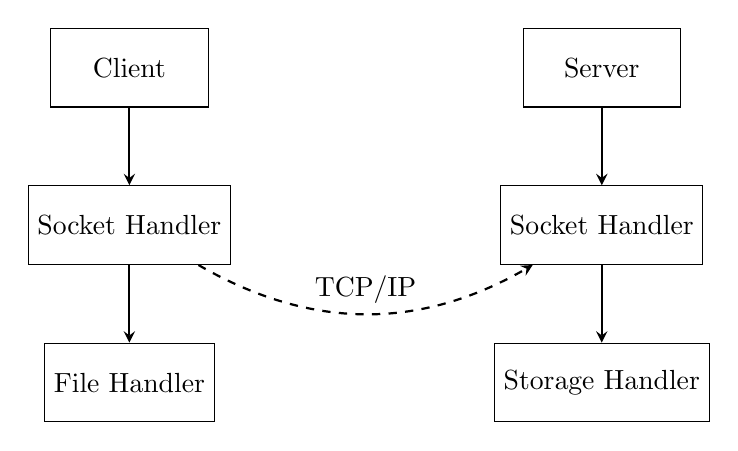
\begin{tikzpicture}[node distance=2cm]
    % Define styles
    \tikzstyle{component} = [rectangle, draw, text centered, minimum width=2cm, minimum height=1cm]
    \tikzstyle{arrow} = [thick,->,>=stealth]
    
    % Components
    \node [component] (client) {Client};
    \node [component, right of=client, xshift=4cm] (server) {Server};
    \node [component, below of=client] (csocket) {Socket Handler};
    \node [component, below of=server] (ssocket) {Socket Handler};
    \node [component, below of=csocket] (filehandler) {File Handler};
    \node [component, below of=ssocket] (storage) {Storage Handler};
    
    % Connections
    \draw [arrow] (client) -- (csocket);
    \draw [arrow] (csocket) -- (filehandler);
    \draw [arrow] (server) -- (ssocket);
    \draw [arrow] (ssocket) -- (storage);
    \draw [arrow, dashed] (csocket) to[bend right] node[above] {TCP/IP} (ssocket);
\end{tikzpicture}
\caption{System Component Organization}
\label{fig:organization}
\end{figure}

\section{Implementation Details}
The implementation uses Python's built-in socket library for network communication. Key features include:
\begin{itemize}
    \item Chunked file transfer (1024 bytes)
    \item Error handling and graceful connection closure
    \item Support for any file type (binary mode)
    \item EOF signaling for transfer completion
\end{itemize}

\section{Task Distribution}
Implementation responsibilities were distributed as follows:
\begin{itemize}
    \item Socket Programming and Network Setup
    \begin{itemize}
        \item Server socket creation and binding
        \item Client connection handling
        \item Protocol implementation
    \end{itemize}
    \item File Operations
    \begin{itemize}
        \item File reading and writing
        \item Chunked transfer implementation
        \item EOF handling
    \end{itemize}
    \item Error Handling and Testing
    \begin{itemize}
        \item Connection error handling
        \item File operation error handling
        \item System testing and verification
    \end{itemize}
\end{itemize}

\section{Usage Instructions}
To use the file transfer system:

\textbf{1. Start the server:}
\begin{lstlisting}[language=Python]
python script.py server
\end{lstlisting}

\textbf{2. Run the client with a file to transfer:}
\begin{lstlisting}[language=Python]
python script.py client filename.txt
\end{lstlisting}

\appendix
\section{Complete Source Code}
The complete implementation is provided below:

\subsection{TCP File Transfer Implementation}
\begin{lstlisting}[language=Python]
import socket
import os
import sys

def start_server(host='localhost', port=12345):
    # Create socket
    server_socket = socket.socket(socket.AF_INET, socket.SOCK_STREAM)
    
    # Bind socket
    server_socket.bind((host, port))
    
    # Listen for connections
    server_socket.listen(1)
    print(f"Server listening on {host}:{port}")
    
    while True:
        # Accept connection
        client_socket, client_address = server_socket.accept()
        print(f"Connection from {client_address}")
        
        try:
            # Receive filename
            filename = client_socket.recv(1024).decode()
            print(f"Receiving file: {filename}")
            
            # Open file for writing
            with open(f"received_{filename}", 'wb') as f:
                while True:
                    # Receive data
                    data = client_socket.recv(1024)
                    if not data or data == b'EOF':
                        break
                    # Write data to file
                    f.write(data)
            
            print("File received successfully")
            
        except Exception as e:
            print(f"Error: {e}")
        
        finally:
            # Close connection
            client_socket.close()

def send_file(filename, host='localhost', port=12345):
    # Create socket
    client_socket = socket.socket(socket.AF_INET, socket.SOCK_STREAM)
    
    try:
        # Connect to server
        client_socket.connect((host, port))
        print(f"Connected to {host}:{port}")
        
        # Send filename
        client_socket.send(filename.encode())
        
        # Check if file exists
        if not os.path.exists(filename):
            raise FileNotFoundError(f"File {filename} not found")
        
        # Open and send file
        with open(filename, 'rb') as f:
            while True:
                # Read data
                data = f.read(1024)
                if not data:
                    # Send EOF marker
                    client_socket.send(b'EOF')
                    break
                # Send data
                client_socket.send(data)
        
        print("File sent successfully")
        
    except Exception as e:
        print(f"Error: {e}")
        
    finally:
        # Close connection
        client_socket.close()

if __name__ == "__main__":
    if len(sys.argv) < 2:
        print("Usage:")
        print("As server: python script.py server")
        print("As client: python script.py client filename")
        sys.exit(1)
    
    mode = sys.argv[1]
    
    if mode == "server":
        start_server()
    elif mode == "client":
        if len(sys.argv) != 3:
            print("Please provide filename for client mode")
            sys.exit(1)
        send_file(sys.argv[2])
    else:
        print("Invalid mode. Use 'server' or 'client'")
\end{lstlisting}

\end{document}